\chapter{Differential Geometry}
As we have noted before general relativity is a inherent local theory. It is convenient to formulate it in terms of differential geometry.
\section{Manifolds}
\begin{definition}
A $n$ dimensional manifold $M$ is a Hausdorff space with countable basis, that
is locally homeomorphic to $\mathbb{R}^n$. We will give a short introduction to
the most important terms.
\end{definition}
\begin{remark}
The requirements Hausdorff and countable basis are of a more technical nature and are satisfied for most of the objects one can imagine 
except some pathological examples (we won't go into the details on this).

Locally homeomorphic to $\mathbb{R}^n$ means there exists a set of \emph{charts} 
$(\varphi,U^\varphi)$ called an \emph{atlas} $\mathcal{A}$ with $\cup_{\varphi\in\mathcal{A}} U^\varphi =M$, 
i.e. the charts cover the whole manifold. The maps $\varphi:U^\varphi\to \varphi(U^\varphi)\subset\mathbb{R}^n $ are homoemorphisms, 
meaning that $U^\varphi$ is open, $\varphi$ is bijective and both $\varphi$ and $\varphi^{-1}$ are continuous.
Further for any two $\varphi,\psi\in \mathcal{A}$, the coordinate changes 
$\varphi\circ\psi^{-1}:\psi(U^\psi\cup U^\varphi)\to \phi(U^\psi\cup U^\varphi)$ be infinitely often differentiable.
\end{remark}
\begin{figure}[htb]
    \begin{center}
        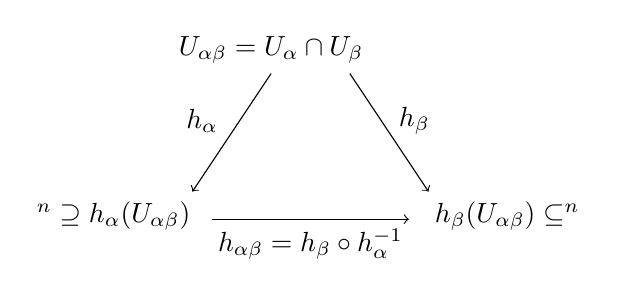
\begin{tikzpicture}
            \draw [->] (1,1.5) -- (0,0);
            \draw [->] (2,1.5) -- (3,0);
            \draw [->] (0.25,-0.35) -- (2.75,-0.35);
            \node [below] at (-1,0) {$\Reals^n \supseteq h_\alpha(U_{\alpha\beta}) $};
            \node [above] at (1,1.5) {$U_{\alpha\beta} = U_\alpha \cap U_\beta$};
            \node [below] at (4,0) {$h_\beta(U_{\alpha\beta}) \subseteq \Reals^n$};
            \node [left] at (0.45,0.9) {$h_\alpha$};
            \node [right] at (2.5,0.9) {$h_\beta$};
            \node [below] at (1.5,-0.35) {$h_{\alpha\beta}= h_\beta \circ h_\alpha^{-1}$};
        \end{tikzpicture}
    \end{center}
    \caption{Coordinate change.} %TODO better caption.
\end{figure}

We can now reduce differentiation on the manifold to the ordinary differentiation in $\mathbb{R}^n$. 
Since physical laws are described in terms of differential equations, we can formulate them on $M$. 
The fact that the coordinate changes are $C^\infty$ ensures that differentiability is well defined (and thus the physical laws are).

\begin{sidenote}[Differentiability depends on the Differential Structure]
There can be different \emph{differential structures} on a manifold, 
which means there are multiple (maximal)alases, which
could not be merged because the coordinate changes would not be $C^\infty$. Those differentiable structures therefore imply different notions of differentiability. 
Remarkably this may even play a role in some physical theories. 
As an example an 11d-supergravity can be described as a product
$\Reals^{3+1}\times \Sphere^7$.
Where $\Sphere^7$ is the 7-sphere and $\Reals^{3+1}$ Mikovski space.
This means on every point in the $\mathbb{R}^{3+1}$ there is a (small) $\Sphere^7$  located that contains additional spatial dimensions. 
The $\Sphere^7$ has 28 different differential structures, so the choice of
such a structure affects the theory for the above reasons.
\end{sidenote}
All simple examples we come of can be embedded in a higher space. The Whitney
embedding theorem states that every real $n$-dimensional Manifold
can be embedded to $\Reals^{2n}$ (This is however not true for complex, i.e. analytic manifolds).
For example the $\Sphere^2$ can be interpreted as submanifold of the $\Reals^3$.
However manifolds are objects that exists independent of such embeddings. 
For example a torus can be thought of as a square with the opposite sides identified (leaving to the left results in re-entering in the left).
\begin{sidenote}[Topology of the Universe]
In addition to the local structure, we may question the global, i.e. the
topological structure of the universe.
On may for example imagine that we live on the surface of a 3-sphere (finite but boundless universe). 
However this might be observable in crosscorelation in the cosmic microwave background from photons reaching us 
from different directions but coming from the same event. There is no evidence of such phenomena so far. 
Most models can be excluded to some certainty. A cylindrical
universe is still possible (finite in one, infinite in the
other directions).
\end{sidenote}
\section{Vectors}
Vectors are important objects describing physics. The naive view as an "arrow pointing frow one point to another" is flawed. 
For example on a sphere an arrow connecting two points does not make much sense.
We want to find a description of vectors as objects that are naturally related to the structure of the manifold independent of the embedding.
\subsection{Definitions}
There are three equivalent definitions for a
vector:
\begin{enumerate}
    \item Algebraic 
    \item Physical
    \item Geometrical 
\end{enumerate}
We start by giving the algebraic definition which is the most
abstract and prefered by mathematicans, because it is suitable for proofs.
Vectors are identified with derivatices, which are formally defined by
\begin{definition}[Derivation]
A derivation $D$ satisfies the following rules for all $f,g\in
C^\infty(M,\Reals)$ and $\lambda \in \Reals$:
\begin{align}
    D(af+bg) &=Df+Dg\\
    D(\lambda f)&=\lambda f\\
    D(fg)&= (Df)g+f(Dg)
\end{align}
\end{definition}
We then define a vector by 
\begin{definition}[Vector,
algebraic] A vector in $p$ is a derivation on the germ at $p$.
\end{definition}
The germ is the set of all functions $f\in C^\infty(M,\Reals)$, where we
identify all functions that are equal in some neighbourhood of $p$, i.e. vectors are local objects.
Given two vectors we can construct a new one, the \emph{Lie bracket}
\begin{equation}
    [X,Y]f:=X(Yf)-Y(Xf)\, .
\end{equation}
The only property that has to be checked is that it satisfies the Leibniz rule.
\begin{equation}
    XY(fg)=X[(Yf)g+f(Yg)]=(XYf)g+(Yf)(Xg)+(Yg)(Xf)+(XYg)f\\
\end{equation}
Subtracting $YX(fg)$ proves that $[X,Y]$ is indeed a vector. The fact that we
have a natural vectorspace structure on the set of vectors at $p$ motivates the
following
\begin{definition}
The Tangentspace $T_pM$ is the space of all vectors in $p\in M$.
\end{definition}
A basis of $T_pM$ is given by the derivation along the
coordinates $\partial_i$, therefore its dimension is equal to that of the manifold $M$.
Proof sketch:
\begin{enumerate}
    \item Show $f(x^i)=f(0)+x^i\tilde{f}(x^i)$
    \item Write $X=a^i\partial_i$
    \item Show $Xf=0\quad \forall f \iff X=0$
\end{enumerate}
Every vector $A$ can be written as $A=A^i\pd{}{{x^i}}$, where $A^i$ are the
components of the vector. We can now look how the components of the vector
transform under a change of coordinates (the vector itself is invariant!). 
We usually denote the elements of the transformed systems with a bar.
By the chain rule we have
\begin{equation}
    A= a^k\pd{}{{x^k}}= a^k\pd{\overline{x}^i}{{x^k}}\pd{}{{\overline{x}^k}}\, .
\end{equation}
We can also express $A$ directly in the new basis
\begin{equation}
    A= \overline{a}^i\pd{}{{\overline{x}^i}}\, .
\end{equation}
Comparing the coefficients gives the vector transformation law
\begin{equation}
    \overline{a}^i=a^k\pd{\overline{x}^i}{{x^k}}\label{eq:coefftrafo}\, .
\end{equation}
\begin{definition}[Vector,
physical] A vector with components $A^i$ is a object that transforms according
to \ref{eq:coefftrafo} under a change of coordinates.
\end{definition}
Consider a curve on $M$, i.e. a map $\gamma:\mathbb{R}\to M$, with
$\gamma(0)=p$, $\dot{\gamma}(0)=X$. Then $D_X f=\od{}{t}(f\circ\gamma)(0)$ is
a derivative, namely the directional derivative along $X$.
For the special curves $\gamma_i(t)=p+te_i$, 
$D_{\dot{\gamma}_i} f=\partial_if$, so we can identify the derivatives with
the geometrical tangent space.

Since we have a basis, we can work in local coordinates.
\begin{example}[Lie brackets in local coordinates]
Let $A=A^i\pd{}{{x^i}}$, $B=B^i\pd{}{{x^i}}$ be vectors, then the Lie bracket
reads
\begin{equation}
    [A,B]^j=A^i\partial_iB^j-B^i\partial_iA^i\, .
\end{equation}
\end{example}
Since the tangent space is a vector space, we can define its dual space
\begin{definition}[Cotangentspace] The Cotangentspace is defined as the set of
linear maps from $T_pM$ to $\mathbb{R}$
\begin{equation}
    T_pM^*=\{L:T_pM\to \mathbb{R}\, |\, L \text{ linear}\}\, .
\end{equation}
\end{definition}
The Cotangentspace is again a vector space of the same dimension. Its elements
are called dual or covariant vectors.
We can define a basis on $	T_pM^*$, which we denote by $\dif x^i$ and  which acts on $T_pM$ via
\begin{equation}
    \dif x^i(\partial_j)=\delta^i_j\, . \label{eq:orthdual}
\end{equation}
It can easily deduced by \eqref{eq:orthdual} that the components of a dual vector transform as
\begin{equation}
    \overline{a}_i=\pd{x^k}{{\overline{x}^i}}a_k\, .
\end{equation}
\begin{remark}[Dual vectors in flat space]
If $\vec{a},\vec{b}\in\mathbb{R}^n$ contain the components of a vector and a
dual vector respectively, then the transformation can be written in matrix form
\begin{align}
    \vec{a}&\to V\vec{a}\, ,\\
    \vec{b}&\to\left(V\transpose\right)^{-1}\vec{b}\, ,
\end{align}
with $V=\left(\pd{\overline{x}^i}{{x^j}}\right)_{ij}$ the
Jacobian of the transformation.
In normal calculus we restrict ourself to orthogonal transformations (i.e.
mapping orthonormal bases onto each other) for which
$\left(O\transpose\right)^{-1}=O$.
Which is the reason why we do not bother to distinguish between vectors and dual vectors because they transform identically. 
In special relativity we have e.g.
$\left(\Lambda\transpose\right)^{-1}\neq\Lambda$ for a boost and the difference
becomes even more important in general relativity where the relation can become arbitrarily complicated.
\end{remark}
\section{Tensors}
From vectors $A$ ,$B$ we can construct new objects with multiple indices that posses well defined transformation behaviour. 
For example consider
\begin{equation}
    \overline{T}^{ij}=a^ib^j\, ,
\end{equation}
which transforms as
\begin{equation}
    T^{ij}=\pd{\overline{x}^i}{{x^k}}\pd{\overline{x}^j}{{x^l}}a^kb^l=\pd{\overline{x}^i}{{x^k}}\pd{\overline{x}^j}{{x^l}}T^{kl}\,
   .\label{eq:tensortrafo}
\end{equation}
We call an object that transforms in this way a \emph{tensor}. 
As with vectors, it is possible to define tensors in a coordinate independent
way.
At this point we will make things easier and only consider the physical
definition, i.e. classify tensors by a transformation according to \eqref{eq:tensortrafo}.

A tensor is said to be symmetric in two indices if it stays invariant when exchanging those indices, e.g.
\begin{equation}
    T_{ab}=T_{ba}\, .
\end{equation}
\begin{remark}
We have not yet established a relation between upper and lower indices, i.e. we have no metric. Expressions of the form
\begin{equation}
    \tensor{T}{^a_b}=\tensor{T}{^b_a}
\end{equation}
make no sense, since they can not be true in every system.
\end{remark}
\section{The Metric}
So far we have not defined a length scale on manifolds yet. We will do so now by
introducing a \emph{metric} 
\begin{definition}[Metric]
A metric $g$ on a manifold $M$, is a non-degenerate ($\det(g)\neq 0$), symmetric
covariant two tensor.
\end{definition}
We have already seen examples of metrics for the flat space, e.g. in spherical coordinates $g$ was given as
\begin{equation}
    g=
    \begin{bmatrix}
        1 & 0\\
        0 & r^2\\
    \end{bmatrix}\,.
\end{equation}
A metric that is positive definite is called \emph{Riemanian metric}. In
relativity we deal with \emph{Lorentzian metrics}, for which there are vectors
beside the zero vector which have zero 'length'. In flat space we have
$\tensor{g}{_i_j}=\tensor{\eta}{_i_j}$.
\begin{remark}[About
raising and lowering indices] Supose we have given a vector $A=A^i\partial_i$
with coodinates $A^i$, then we can relate it 
in a natural way to a linear form $g(A,\cdot)$,
\begin{equation}
\begin{split}
 g(A,\cdot)\,\colon T_pM &\to \Reals\\
 X &\mapsto g(A,X)
\end{split}\, ,
\end{equation}
i.e. a dual vector. The components of this dual vector are given by its action
on the Basis elemts of the tangentspace
\begin{equation}
A_i=g(A,\partial_i)=A^jg(\partial_j,\partial_i)=g_{ji}A^j\,,
\end{equation}
which is exactly the law for lowering indices. Given the inverse metric we can
multiply this equation by it to obtain $A^i$ in terms of $A_i$.
\end{remark}
\section{Parallel Transport}
Idea: Generalize parralel transport from flat space.
(PICTURES) 
If we express a vector in non-cartesian coordinates and shift it it's
coordinates do not change.
We take a look on two operations:
\begin{enumerate}
\item the change of the vector itself
\item the change of its coordinates
\end{enumerate}
Let $A_i$ be the coordinates of a vector in a system $x^i$ and $B_i$ the in a
system associated with coordinates $y^i$ respectively.
\begin{equation}
A_i\pd{{y^j}}{{x^i}}B_j\, ,\quad B_i\pd{{x^j}}{{y^i}}A_j\, .
\end{equation}
We look at vectors whose coodinates in the system $y^i$ do not change i.e.
$\delta B_i=0$ The variation of $A_i$ is given by
\begin{equation}
\delta
A_i=\delta\left(\pd{{y^j}}{{x^i}}\right)B_j
=\md{{y^j}}{2}{{x^i}}{}{{x^k}}{}\delta
x^k B_j\, .
\end{equation}
Expressing $B_i$ in terms of $A_i$ yields
\begin{equation}
\delta A_i = \md{{y^j}}{2}{{x^i}}{}{{x^k}}{}\pd{{x^l}}{{y^j}}A_l\delta x^k
=:\affin{l}{i}{k}A_l\delta x^k
\end{equation}
$\affin{l}{i}{k}$ is called \emph{affine connection} or short affinity.
\begin{remark}
We can always find a coordinate system in wich $\affin{l}{i}{k}\equiv 0$, this
system is called \emph{Riemanian normal coordinate system} (RNCS).
\end{remark}
We notice that if 
\begin{equation}
\left(\pd{{A_i}}{{x^j}}-\affin{l}{i}{k}A_l\right)\delta x^k = 0\,
,\label{eq:covdev}
\end{equation}
The vector $A$ does not change its cordinates. We define a \emph{covariant
derivative} 
\begin{equation}
\tensor{A}{_i_;_j}:=\tensor{\nabla}{_j}\tensor{A}{_i}:=\pd{{A_i}}{{x^j}}-\affin{l}{i}{k}A_l\,
.
\end{equation}
It can easyly be seen that the covariant derivative of a tensor transforms as a
tensor, by inspecting \eqref{eq:covdev} and applying the quotient theorem.
\begin{remark}[The
Covariant Derivative in Electrodynamics] Example from Electrodynamics concerning the covariant derivative. 
The theory is invariant under transformations $\phi\to e^{\imI \alpha}\phi$, 
because $\phi^*\phi$ and $\phi^*\nabla\phi-\phi\nabla\phi^*$ do not change.
Vervollständigen\ldots
\end{remark}
Since we have now established a relation between vectors and dual vectors, we
can also determine the covariant derivative of a dual vector. Therefore we
consider the scalar $A_iB^i$. Since the covariant derivative satisfies the
Leibniz rule we get
\begin{align}
\tensor{(A_iB^i)}{_{;j}} =
\tensor{A}{_i_;_j}\tensor{B}{^i}+\tensor{A}{_i}\tensor{B}{^i_;_j}
\end{align}
But for scalars the covariant derivative is identical to the normal derivative
so that 
\begin{align}
(A_iB^i)_{;j} =(A_iB^i)_{,j}=
\tensor{A}{_i_,_j}\tensor{B}{^i}+\tensor{A}{_i}\tensor{B}{^i_,_j}
\end{align}
If we put in the covariant derivative of a we get 
\begin{equation}
\tensor{A}{_i}\tensor{B}{^i_;_j}=\tensor{A}{_i}\left(\pd{}{{x^j}}B^i+\Gamma^i_{kj}\tensor{B}{^k}\right)
\end{equation}
Since $A$ was arbitary, we can deduce that
\begin{equation}
\tensor{B}{^i_;_j}=\left(\pd{}{{x^j}}B^i+\Gamma^i_{kj}\tensor{B}{^k}\right)
\end{equation}
for a (1,1)-tensor we get:
\begin{equation}
\tensor{A}{^i_j_;_k}=\pd{}{{x^k}}\tensor{A}{^i_j}-\Gamma^a_{jk}\tensor{A}{^i_a}+\Gamma^i_{ak}\tensor{A}{^a_j}\,
.\end{equation}
Similar expressions hold for tensors of arbitary rank where each index gives an
aditional term containing a contraction with the affinity $\Gamma^i_{jk}$. 
We now want to consider curved spaces. This can not immediatly be determined by
the metric, for example the polar coordinates do not look flat even though they
describe the ordinary $\Reals^2$. (PICTURES)
\subsection{Riemanian Curvature Tensor}
\ldots
We can contract indices on the Rieman Tensor
\begin{equation}
\tensor{R}{^i_i_k_l}=\pd{{\Gamma^i_{il}}}{{x^k}}-\pd{{\Gamma^i_{ik}}}{{x^l}}
\end{equation}
which is zero for a metric affinity. The Ricci tensor is given by
\begin{equation}
\tensor{R}{_j_k}=\tensor{R}{^i_j_k_i}\, .
\end{equation}
Because of the symmetrie this are all independent contractions. Notice that at
this point we cannot raise or lower indices to contract different indices.
Since we can express the Rieman tensor in terms of commutators ther is a also a
symmetry that can be derived from the Jacobi identity:
Physics can be described in terms of differential equations. We for example
would like to have a object similiar to the laplacian in curved coordinates.
However $\partial_i\partial_i$ is not coordinate invariant. We therefore
introduce a metric. The equivalence principle implies that space is locally
Minkovski.
\begin{sidenote}
There are several theories that do not need a metric. For example 3d gravity.
\end{sidenote}
Inner product 
\begin{equation}
\langle A,B\rangle=\tensor{g}{_i_j}\tensor{A}{^i}\tensor{B}{^j}
\end{equation}
Pseudo norm
\begin{equation}
\|A\|^2=\langle A,A\rangle=\tensor{g}{_i_j}\tensor{A}{^i}\tensor{A}{^j}
\end{equation}
Since the connection and the metric are not related, we stil don't have a lenght
scale on the manifold
\begin{equation}
\tensor{R}{_i_j_k_l}:=\tensor{g}{_i_a}\tensor{R}{^a_j_k_l}
\end{equation}
Only useful if $R$ and $g$ are related i.e. metric connection.
(Bilder)
A curve is a map $\gamma:\Reals\to M$. The parametrisation is arbitary e.g.
\begin{equation}
\begin{split}
\gamma:\, &\Reals\to \Reals^2\\
& t\mapsto
\frac{1}{2} t^2
\begin{bmatrix}
1 \\
1
\end{bmatrix}
\end{split}\, ,
\end{equation}
clearly describes a straight line with $y=x$ 